\chapter{Background}\label{ch2}

In this chapter, the foundations of the thesis are elaborated. We formally define methods, concepts and tools used. Starting with the description of the 3D Morphable Model (3DMM) \cite{Blanz:1999:MMS:311535.311556, Romdhani3DM} that we utilize, followed by an explanation of a novel fully probabilistic  method
to interpret a single face image with the 3DMM\cite{Schoenborn2017}. As well as, the important characteristics of the depth cameras. 

\section{3D Morphable Model}
The 3DMM is a fully parametric generative face model constructed from 200 high quality face scans. The model contains probabilistic PCA (PPCA) models for shape, color and expression \cite{8373814, EGGER2017115}.  In a traditional PCA-based settings the shape S, color C and facial expression E models are constructed through the parameter set $\theta=\{\theta_S, \theta_C, \theta_E\}$ as follows:
\begin{equation}
    \begin{split}
    S(\theta) &= \mu_S + U_S D_S \theta_S + \mu_E + U_E D_E \theta_E \\
    C(\theta) &= \mu_C + U_C D_C
    \end{split}
\end{equation}
Where $\mu$ denotes the mean of the corresponding model, $U$ is a matrix that contains the principal components, and $D$ denotes a diagonal matrix consisting of the variances along the principal directions. The expression model here, is modeled as a deformation of the neutral (mean) face shape. In a probabilistic setting the shape and color models are transformed into a distribution of shape $P(S \mid \theta)$ and color $P(C \mid \theta)$ components with the additive Gaussian noise\cite{ALBRECHT2013959, EGGER2017115}:

\begin{equation}
    \begin{split}
    P(S \mid \theta) &= \mathcal{N}(S \mid \mu_S + U_S D_S \theta_S + \mu_E + U_E D_E \theta_E, \sigma_S^2 I) \\
    P(C \mid \theta) &= \mathcal{N}(C \mid \mu_C + U_C D_C, \sigma_C^2 I)
    \end{split}
\end{equation}

The parameter set $\theta$ follow a standard normal distribution in latent vector space\cite{EGGER2017115} which is also defined outside the linear span of 200 scans:

\begin{equation}
    P(\theta) = \mathcal{N}(\theta \mid 0, I)
\end{equation}
To generate realistic 3DMM instances (Figure \ref{f2.1}) and render synthetic face images $\mathcal{I}$, parameter set $\theta$ contains an additional camera $\theta_P$ and illumination $\theta_L$ parameters that are modeled separately from the other three. 

\begin{figure}
    \centering
    \captionsetup{labelformat=empty}
    \begin{minipage}{.32\textwidth}
        \centering
        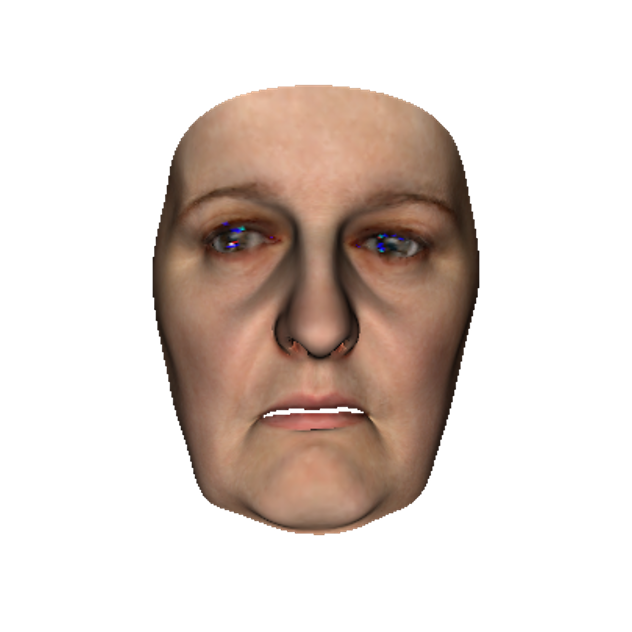
\includegraphics[width=\textwidth]{Figures/Pictures/rs1_t.png}
        \caption*{Sample}
      \end{minipage}
    \begin{minipage}{.32\textwidth}
      \centering
      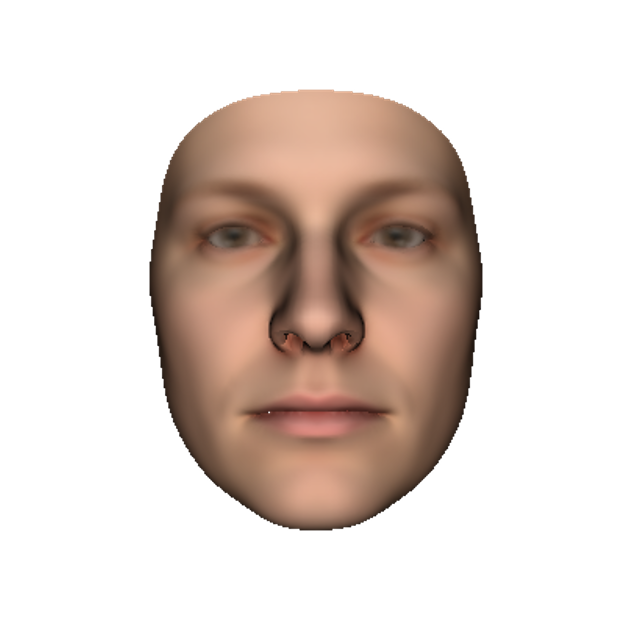
\includegraphics[width=\textwidth]{Figures/Pictures/mean_t.png}
      \caption*{Mean}
    \end{minipage}
    \begin{minipage}{.32\textwidth}
        \centering
        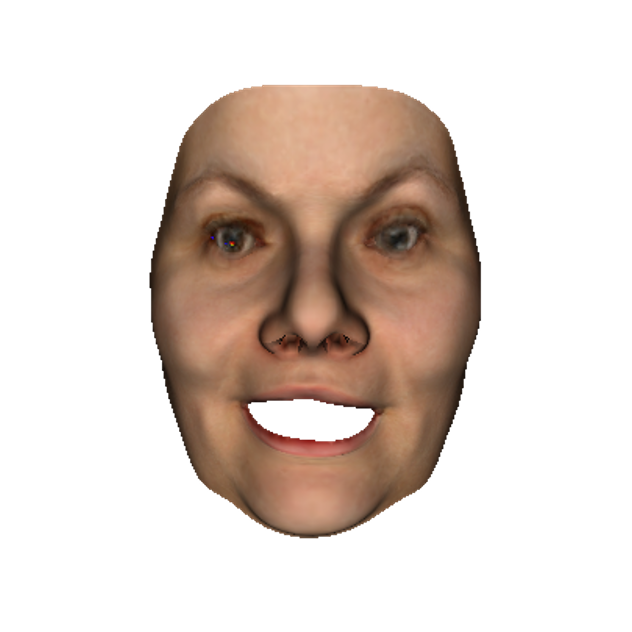
\includegraphics[width=\textwidth]{Figures/Pictures/rs2_expr_t.png}
        \caption*{Sample with expression}
    \end{minipage} 
      \captionsetup{labelformat=default}   
      \caption{3DMM face model instances.}
      \label{f2.1}
\end{figure}

This allows us to synthesize the real world appearance of the face. By tuning all the mentioned parameters, we can approximate the appearance of the synthetic face to the target face. Besides parameter space, the model is also able to take care of the image rendering process $\Re$ which renders an image $\mathcal{I}(\theta)$ based on given parameters through 
\begin{equation}
    \mathcal{I}(\theta) = \Re(\mathcal{M}(\theta_S, \theta_C, \theta_E); \theta_P, \theta_L).
\end{equation}    
The 3DMM model also has a set of modified model versions that are either restricted to a certain region or are down-scaled, low-resolution versions\footnote{Down-scaled versions usually have a lesser number of points and triangles hence are less flexible, but they perform the mesh operations faster} of the original model. The model restricted to a certain region is important for domain specific applications that only utilize specific parts of the model. For example, we use the model (Figure \ref{f2.2}) from \cite{Schoenborn2017} which only covers the face region and discards other parts like ears, neck, and part of the forehead. 

\begin{figure}
    \centering
    \begin{minipage}{.32\textwidth}
        \centering
        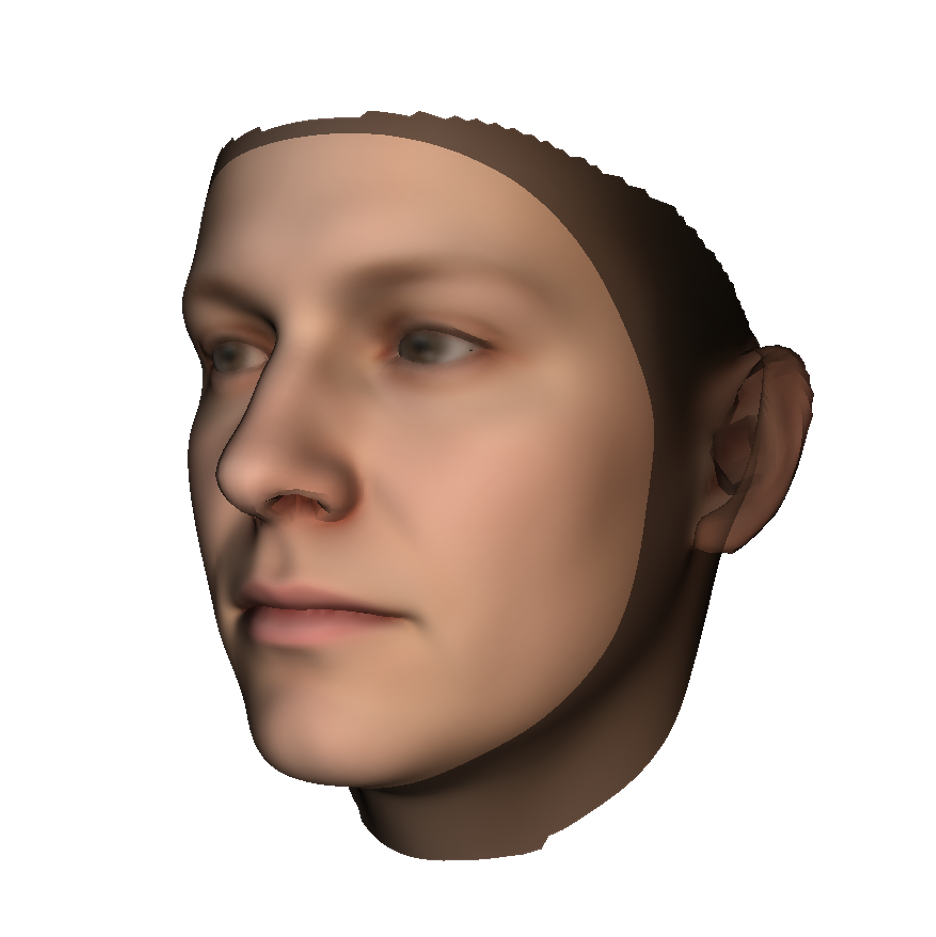
\includegraphics[width=\textwidth]{Figures/Pictures/sideA_t.png}
      \end{minipage}
      \begin{minipage}{.33\textwidth}
          \centering
          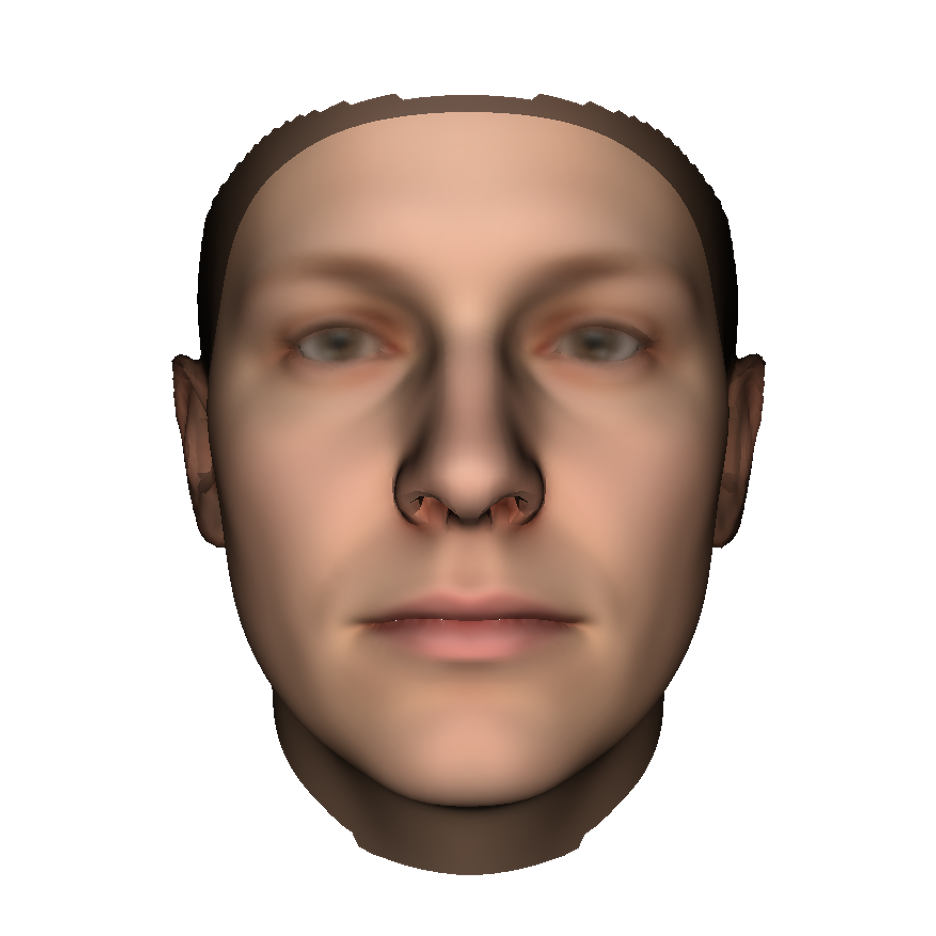
\includegraphics[width=\textwidth]{Figures/Pictures/face_bfm_close_t.png}
    \end{minipage}
    \begin{minipage}{.32\textwidth}
        \centering
        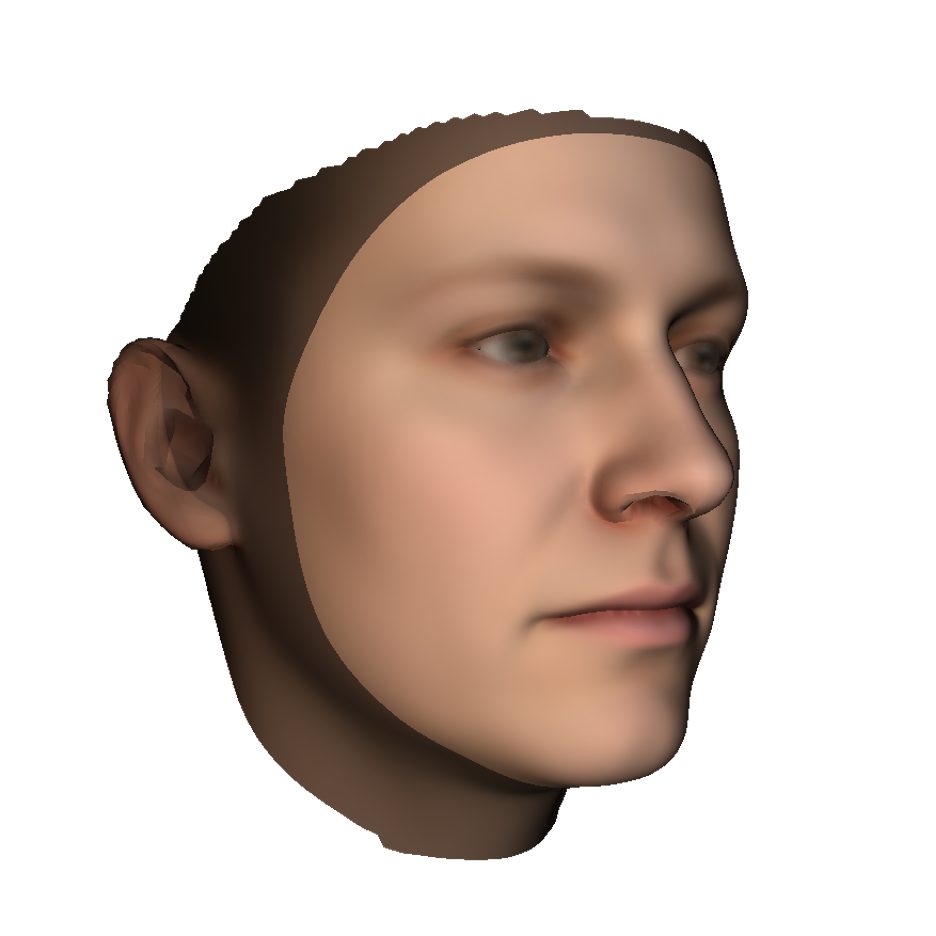
\includegraphics[width=\textwidth]{Figures/Pictures/sideB_t.png}
    \end{minipage}
    \caption{Restricted face model displayed over the full model(dark)}
    \label{f2.2}
\end{figure}

Beneficially to our application, this restriction also ignores parts of the model that are too complex, noisy or low quality, for example ears, that could potentially cause some problems during the fitting.
\section{Fitting Pipeline}
Having the flexible Parametric Appearance Model (PAM) as a basis of the fitting framework allows us to model a variety of real world scenes with challenging illumination conditions. In this section, we explain how standard fitting pipeline and its augmented variant utilizes Markov Chain Monte Carlo sampling to perform approximate inference.\bigskip  

\subsection{Markov Chain Monte Carlo (MCMC)}\label{s2.2.1}
To generate parametric face instances, the Analysis-by-Synthesis method employs a probabilistic image analysis using Bayesian inference. Formally, the fitting pipeline is a procedure that for any given face image returns a model fit which best corresponds to the face in the input image. It is important to note that commonly applications aim to obtain a single solution as a result, however, this is not the case for fitting pipeline. Instead of aiming for a single solution the fitting pipeline produces a posterior distribution of possible solutions. Since the true posterior distribution is unknown, the fitting process needs to approximate it. To perform approximate inference in this setting the Metropolis-Hastings (MH) algorithm is used. The algorithm is a method of Markov Chain Monte Carlo sampling and it is especially useful when sampling from distributions from which direct sampling is not feasible. The algorithm is an iterative process that draws random samples $\theta'$ from a proposal distribution $Q(\theta'\mid\theta)$ that are being evaluated based on their likelihood value. In the figure bellow single step of MH algorithm is shown.\bigskip

\begin{algorithm}[H]
    \SetAlgoLined
     $\bullet$ Initialize sample $\theta \sim Q(\theta)$\;
     $\bullet$ Generate the next sample with current sample $\theta$:\\
     {\addtolength{\leftskip}{5mm}
     1. Propose a sample $\theta'$ based on current sample: $\theta'\sim Q(\theta'\mid\theta)$\;
     2. With probability: $\alpha = min\Big\lbrace\frac{P(\theta')}{P(\theta)}\frac{Q(\theta\mid\theta')}{Q(\theta'\mid\theta)}, 1\Big\rbrace$ accept or reject samples\;

      3. If sample $\theta'$ is accepted set $\theta'$ to be a new state $\theta$, otherwise keep $\theta$ unchanged\; 
     }
     \caption{Metropolis-Hastings algorithm}
     \label{a1}
\end{algorithm}\bigskip

The two principal parts of the algorithm are the proposal distribution $Q$ from which samples are drawn and the likelihood estimation $P(\theta)$. Let us describe both of these key components in detail.  \bigskip

The proposal distribution should be simple enough to draw random samples from it. In the settings of the fitting pipeline commonly used proposal distribution is a simple Gaussian random walk proposal distribution: 

\begin{equation}
   Q(\theta'\mid\theta) = \mathcal{N}(\theta'\mid\theta, \sigma^2 I_d). 
   \label{2.5}
\end{equation}

Where $d$ stands for the dimension and $\sigma$ controls the step size the algorithm makes at each sampling iteration. In the fitting pipeline we usually have more than one proposal distributions for each 3DMM parameter update $\theta = \{\theta_S, \theta_C, \theta_E\, \theta_P, \theta_L\}$. Therefore, in practice, $Q(\theta'\mid\theta)$ consists of multiple proposal distributions $Q_i$ combined into one mixture proposal distribution:

\begin{equation}
    Q(\theta' | \theta) = \sum_i c_i Q_i(\theta'|\theta), \sum_i c_i = 1.
    \label{eq2.3}
\end{equation} 

Where $\theta$ is a current sample, $\theta'$ is a newly proposed sample drawn from a proposal distribution $Q_i$, and $c_i$ coefficient controls how often samples are being drawn from the specific $Q_i$ distribution\cite{Schoenborn2017}.\bigskip

The second key part of the MH algorithm is a likelihood estimation term $P(\theta)$ commonly written as $P(\theta\mid\mathcal{I})$. It determines a posterior belief of the current sample parameter set $\theta$ conditioned on the target image $\mathcal{I}$. Computing the posterior directly is not possible, therefore, we employ the classical Bayes' theorem\footnote{Bayes' theorem — \url{https://en.wikipedia.org/wiki/Bayes'\_theorem}} to approximate it based on the prior knowledge $P(\theta)$ and an image likelihood $P(\mathcal{I}\mid\theta)$:

\begin{equation}
    P(\theta \mid \mathcal{I}) = \frac{P(\theta)P(\mathcal{I}\mid \theta)}{\int P(\mathcal{I}\mid \theta)P(\theta)d\theta}
\end{equation}

In this setting finding a single solution then becomes a problem of a maximum-a-posteriori (MAP) inference, which is finding the parameters with the highest posterior probability\cite{10.1007/978-3-642-40602-7_11}. Since we are only interested in the ratio of two different likelihoods $P(\theta\mid\mathcal{I})$ and $P(\theta'\mid\mathcal{I})$ the normalization term can be ignored, and we can rewrite the above formulation as:

\begin{equation}
    P(\theta | \mathcal{I}) \propto P(\theta)P(\mathcal{I} | \theta)
    \label{eq2.5}
\end{equation}

The prior probability $P(\theta)$ of the model estimate $\theta$ is usually defined as a normal distribution: 
\begin{equation}
    \label{eq3}
    P(\theta) = \mathcal N(\theta | 0, \mathcal I).
\end{equation}

The only missing part of the Equation \ref{eq2.5} than is an image likelihood $P(\mathcal{I}\mid\theta)$ which can be reformulated as $P(\mathcal{I}\mid\theta) = \mathcal{L}(\theta;\mathcal{I})$ with equation \ref{eq2.5} transforming to:

\begin{equation}
    \label{eq2.5}
    P(\theta | \tilde{\mathcal I}) \propto \mathcal L(\theta;\tilde{\mathcal I})P(\theta)
\end{equation} 
An image $\mathcal{I}$ that appears in likelihood term means that during the fitting target image is treated as an observation of the 3DMM model instance.
Depending on the phase the fitting pipeline is in, a combination of likelihood functions is used. We briefly discuss the most important likelihood functions used in the fitting pipeline alongside with the phase they are used in.   

\subsection{Landmark Fitting}
During the starting phase of the fitting, it is important to have good pose estimation parameters since the pipeline is crucially dependent on it. If the pose is wrong, the rest of the model parameters cannot be inferred reliably. To deal with this problem, the standard fitting pipeline relies on the landmark fitting phase. During this phase fitting only modifies 3DMMs $\theta_P$ and $\theta_S$ parameters. It does so by evaluating a set of landmark point locations $x_i$ detected (by detection algorithm or manually) onto the target image and projected to the model instance using computer graphics. The projection method uses a pinhole camera model to align model instance to the target face by applying a rotation and translation parameters and then render individual landmarks onto the image plane. By treating those points as an observation of corresponding model points, the algorithm evaluates them using isotropic Gaussian likelihood function: 

\begin{equation}
\mathcal L(\theta; x_1, x_2,\dots, x_N) = \prod_{i=1}^{N} \mathcal N(x_i\mid y_i(\theta), \sigma^2_{LM} I_2) \text{\cite{Schoenborn2017}}.
\label{lmeval}
\end{equation}

Where $x_i$ are observed landmark positions and $y_i(\theta)$ are model landmark positions based on $\theta$. Proposed samples with new camera and shape parameters are getting accepted or rejected based on its likelihood value according to the procedure discussed earlier in Algorithm \ref{a1}. Pose parameters that are part of $\theta_P$ are a combination of Euler rotation angles \textit{\{yaw, nick, roll\}}, translation vector $\vec{t} = \{t_x, t_y, t_z\}$ with $t_z$ indicating the distance from the camera, and scaling parameter to control the focal length of the camera. The proposal distribution (Equation 
\ref{eq2.3}) for landmark fitting consists of a mixture distribution over shape and camera (pose) parameter update proposals. As discussed previously, shape parameters $\theta_S$ are PCA coefficients of the low-rank expansion of the Gaussian Process\cite{8010438} model that are proposed by a weak isotropic Gaussian perturbation proposal\cite{Schoenborn2017}.  The described process adjusts the pose and at the same time makes initial shape correction. Landmark fitting is usually a very fast process since the only few landmark points (usually less than 10) are getting evaluated at a time.

\subsection{Color Fitting}

After the landmark fitting phase the pose of the model instance usually fits well with the target face in the image and the model instance is ready to be utilized for color, illumination and optionally expression proposals as well as shape update proposals. Thus, during the color fitting phase the mixture proposal $Q(\theta'\mid\theta)$ will be a combination of all the above mentioned parameter proposals with various step size and drawing probability as of Equation \ref{eq2.3}. To evaluate proposed samples in this phase the standard fitting pipeline together with landmark evaluation (Equation \ref{lmeval}) relies on independent pixel evaluator likelihood which distinguishes foreground and background pixels\cite{Schonborn:2015:BMG:2798342.2798359} and is formulated as follows:

\begin{equation}
    \mathcal L \left (\theta; \tilde{\mathcal I} \right )
= \prod_{i \in \mathcal F} \mathcal N \left( \tilde{\mathcal I}_i \,\middle |\, \mathcal I_i(\theta), \sigma^2 I_3 \right ) \prod_{i \in \mathcal B} \mathcal L_{\text{BG}}\left ( \tilde{\mathcal I}_i \right ).
\label{eq2.7}
\end{equation}

Where the first product evaluates foreground pixels $i\in\mathcal F$ and second product evaluates background pixels $i\in\mathcal B$. The motivation behind incorporating background pixels into this likelihood and not ignoring them is that, when they are ignored, their likelihood value is assumed to be 1, which is not necessarily true in most cases. \bigskip

So called propose-and-verify flow of the initial architecture of the Metropolis-Hastings algorithm used by \cite{Schoenborn2017, Schoenborn2014} is shown in Figure \ref{f2.3}. As we have mentioned previously, the architecture only uses color image and 2D landmarks as an input. 

\begin{figure}
    \centering
    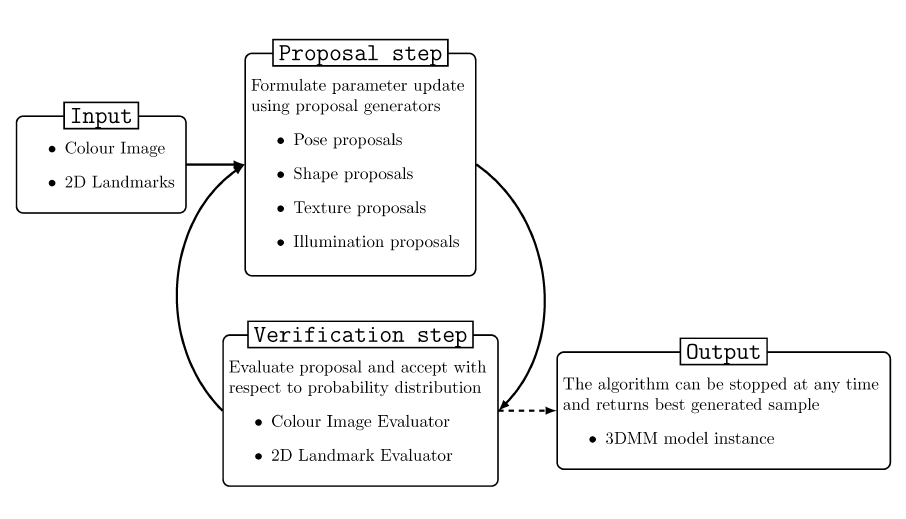
\includegraphics[width=0.85\textwidth]{Figures/flow1.PNG}
    \caption{The architecture of the MH algorithm used by \cite{Schoenborn2017} taken from \cite{betschard2016}}.
    \label{f2.3}
\end{figure}

An augmented version of this flow by \cite{betschard2016} can be seen in Figure \ref{f2.4}, where authors introduced additional depth image and 3D landmark input sources, with respective evaluators. \bigskip

\begin{figure}
    \centering
    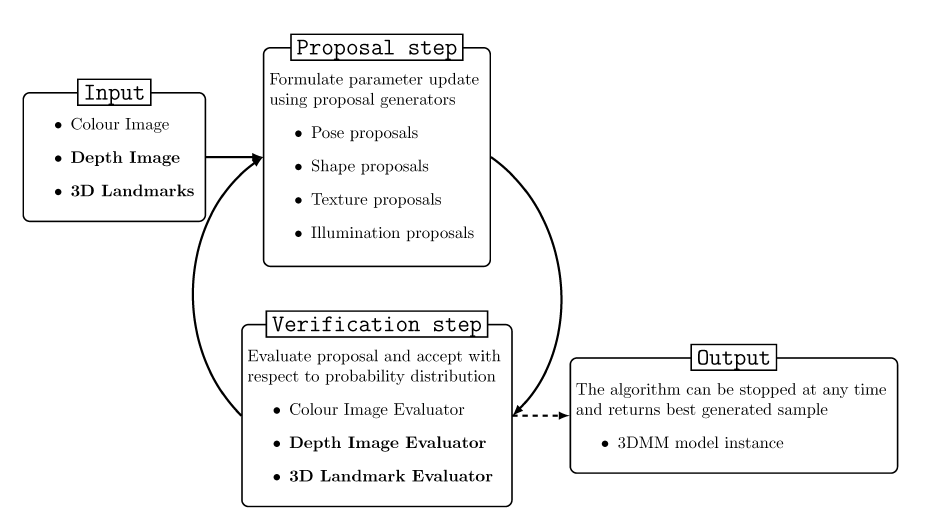
\includegraphics[width=0.85\textwidth]{Figures/flow2.PNG}
    \caption{Augmented MH architecture proposed by \cite{betschard2016}, changes made in the architecture are in bold.}
    \label{f2.4}
\end{figure}

We introduce an alternative way of dealing with this architecture. Instead of using just a depth image (only z-Buffer) we construct a triangle mesh from a point cloud obtained using the depth camera. Details of this process are described in Section \ref{s3.3.3}. We were also forced to find a work-around way to obtain 3D landmarks (Section \ref{s3.3.2}), since they are not provided by the camera SDK anymore. We split the standard fitting pipeline into two sub-fitting pipelines, one that deals with the shape and pose parameter estimation hereafter referred to as \textit{shape fitting module} and the other with color, illumination, and expression with slight shape and pose parameter updates hereafter referred as \textit{color fitting module}. Both of these modules are described in Section \ref{s3.4}.

\section{Depth Camera}

Inferring the exact size of an object when analyzing color images is a challenging task, there is no effective way to reliably recover this information based on color intensities. The depth camera helps us to resolve this issue by providing a distance measure for each pixel (if it is available). There are a few different ways distance is obtained by the depth cameras. One of the algorithms commonly used (and the one our camera uses) to calculate distance is the depth from stereo algorithm better known as \textbf{Stereoscopic Vision}\footnote{\url{https://en.wikipedia.org/wiki/Computer_stereo_vision}} which is a realization of a natural Binocular vision. The basic idea behind Stereoscopic vision is to estimate the distance from the camera to each point by calculating disparities between two parallel view-ports\cite{serg, DBLP:journals/corr/KeselmanWGB17} (Figure \ref{f2.5}). View-port parallelism is achieved with the traditional Image Rectification\footnote{\url{https://en.wikipedia.org/wiki/Image_rectification}} approach, which transforms images onto a common virtual image plane and makes sure that two view-port points are matching. 

\begin{figure}
    \centering
    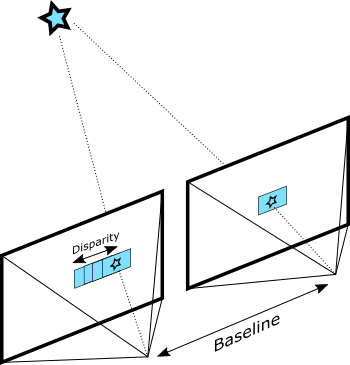
\includegraphics[width=0.55\textwidth]{Figures/Pictures/stereo-ssd-1.png}
    \caption{Depth from stereo. Visualizing two separate view-ports that are being used to calculate disparities. Source: Intel}
    \label{f2.5}
\end{figure}
 
\subsection{De-projection}
Pixel-to-Point and Point-to-Pixel de-projection is a common use-case in computer vision. When needed this feature offers pixel to point mapping and vice-versa by relying on cameras' depth information and intrinsic parameters. Successful de-projection is based on the traditional pinhole camera model \cite{Hartley:2003:MVG:861369} shown in Figure \ref{f2.6}. 

\begin{figure}[h]
    \centering
    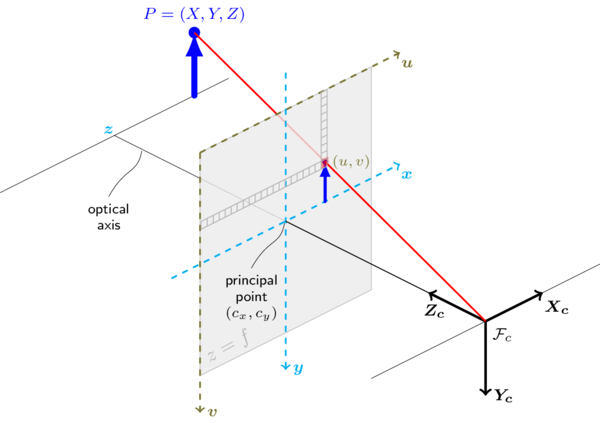
\includegraphics[width=\textwidth]{Figures/pcm.png}
    \caption{Pinhole camera model. $\mathcal F_c$ is the center of the camera, (X, Y, Z) are coordinates of a 3D point in the world coordinate system, ($u$,$v$) are coordinates of a respective point projection in pixels, ($c_x, c_y$) indicates principal points usually located at the image center.  Source: \url{https://docs.opencv.org}}
    \label{f2.6}
\end{figure}


The problem of point to pixel projection is formulated as follows. Given a 3D point coordinates $P_{3D}(X, Y, Z)$ with camera intrinsic parameters\footnote{\url{https://github.com/IntelRealSense/librealsense/blob/master/include/librealsense2/h/rs\_types.h\#L55}} containing ($width$, $height$, $ppx$, $ppy$, $f_x$, $f_y$), calculate the respective pixel coordinates $P(u, v)$ with no distortion introduced. Where in camera parameters, $width$ and $height$ are image dimensions in pixels, $ppx$ and $ppy$ are the horizontal and vertical coordinate of the principal point of the image given as an offset from the left and top edge respectively, and the $f_x$ and $f_y$ are the focal lengths of the image as a multiple of pixel width and height. The focal length is usually the distance from the center of the camera to the image plane also known as the focal plane. It is shown as gray square in Figure \ref{f2.6}.  Once we have all these variables, then the $u$ and $v$ pixel coordinates of $P(u, v)$ are calculated as follows:

\begin{equation}
    \begin{split}
    &x' = \frac{X}{Z}\\
    &y' = \frac{Y}{Z}\\
    &u = x' \cdot f_x + ppx\\
    &v = y' \cdot f_y + ppy\\
    \end{split}
\end{equation}

On the other hand, the problem of de-projecting pixel coordinates into the 3D coordinate space to obtain a 3D point is formulated as follows. Given a pixel coordinates $P(u, v)$ and depth information $d = Z$ alongside the camera parameter set mentioned previously with no distortion introduced, compute the corresponding $P_{3D}(X, Y, Z)$ point in the 3D space. Then $P_{3D}(X, Y, Z)$ coordinates are being calculated as follows:

\begin{equation}
    \begin{split}
    &x' = \frac{u - ppx}{fx}\\
    &y' = \frac{v - ppy}{fy}\\
    &X = d \cdot x'\\
    &Y = d \cdot y'\\
    &Z = d
    \end{split}
\end{equation}

Both techniques we have discussed are already implemented in the camera SDK for us, therefore, throughout the project, we make use of those default methods provided by the SDK.



